\documentclass[14pt,aspectratio=169,xcolor=dvipsnames]{beamer}
\usetheme{SimplePlus}
\usepackage{booktabs}
\usepackage{minted}
\usepackage{mathtools}

\title[short title]{Clase 13: Python científico II}
\subtitle{}
\author[NA Barnafi] {Nicolás Alejandro Barnafi Wittwer}
\institute[UC|CMM] 
{
    Pontificia Universidad Católica de Chile \\
    Centro de Modelamiento Matemático
}

\titlegraphic{
    \vspace{-1.8cm}
    \begin{flushright}
      
\includegraphics[height=2.5cm]{../images/logos/puc.png} 
    \end{flushright}
}

\date{11/09/2024}
%\setbeamercovered{transparent}

\begin{document}
%%%%%%%%%%%%%%%%%%%%%%%%%%%%%%%%%%%%%%%%%%%%%%%%%%%%%%%
\begin{frame}
    \maketitle
\end{frame}
%%%%%%%%%%%%%%%%%%%%%%%%%%%%%%%%%%%%%%%%%%%%%%%%%%%%%%%
\begin{frame}\frametitle{Temas}
    \begin{itemize}
        \item Random, Statistics
        \item Scipy
        \item Pandas
    \end{itemize}

    \vspace{1cm}
    Todas instalables con \code{pip}
\end{frame}
%%%%%%%%%%%%%%%%%%%%%%%%%%%%%%%%%%%%%%%%%%%%%%%%%%%%%%%
\begin{frame}[fragile]\frametitle{\texttt{random}}
    \begin{minted}{python}
  > import random
  > random. # Tab
random.BPF           random.SystemRandom( random.gammavariate(   random.paretovariate( random.seed(           
random.LOG4          random.TWOPI         random.gauss(          random.randbytes(     random.setstate(         
random.NV_MAGICCONST random.betavariate(  random.getrandbits(    random.randint(       random.shuffle(          
random.RECIP_BPF     random.choice(       random.getstate()      random.random()       random.triangular(       
random.Random(       random.choices(      random.lognormvariate( random.randrange(     random.uniform(          
random.SG_MAGICCONST random.expovariate(  random.normalvariate(  random.sample(        random.vonmisesvariate( 
    \end{minted}
    
\end{frame}
%%%%%%%%%%%%%%%%%%%%%%%%%%%%%%%%%%%%%%%%%%%%%%%%%%%%%%%
\begin{frame}[fragile]\frametitle{\texttt{statistics}}
    \begin{minted}{python}
  > import statistics as st
  > st. # Tab
st.Counter(          st.bisect_left(  st.fabs(           st.hypot(              st.median(         st.namedtuple( st.repeat(
st.Decimal(          st.bisect_right( st.fmean(          st.itemgetter(         st.median_grouped( st.numbers     st.sqrt(
st.Fraction(         st.correlation(  st.fsum(           st.linear_regression(  st.median_high(    st.pstdev(     st.stdev(
st.LinearRegression( st.covariance(   st.geometric_mean( st.log(                st.median_low(     st.pvariance(  st.tau
st.NormalDist(       st.erf(          st.groupby(        st.math                st.mode(           st.quantiles(  st.variance(
st.StatisticsError(  st.exp(          st.harmonic_mean(  st.mean(               st.multimode(      st.random      
    \end{minted}
    Compatible con arreglos de \code{numpy} 
\end{frame}
%%%%%%%%%%%%%%%%%%%%%%%%%%%%%%%%%%%%%%%%%%%%%%%%%%%%%%%
\begin{frame}\frametitle{}
    \idea{Consola...}
\end{frame}
%%%%%%%%%%%%%%%%%%%%%%%%%%%%%%%%%%%%%%%%%%%%%%%%%%%%%%%
\begin{frame}\frametitle{Scipy}
    \begin{itemize}
        \item Librería científica
        \item Tiene \emph{muchas} operaciones matemáticas
        \item Álgebra lineal (más eficiente que Numpy)
        \item {\only<2>{\bf}Interpolación de datos}
        \item {\only<2>{\bf}Solución de ecuaciones}
        \item {\only<2>{\bf}Minimización de funciones}
        \item Y MUCHO más
    \end{itemize}

    \begin{flushright}
        
\includegraphics[width=0.2\textwidth]{../images/logos/scipy.png}
    \end{flushright}
\end{frame}
%%%%%%%%%%%%%%%%%%%%%%%%%%%%%%%%%%%%%%%%%%%%%%%%%%%%%%%
\begin{frame}\frametitle{Scipy: Interpolación de datos}
    \only<1>{
        \begin{center}
            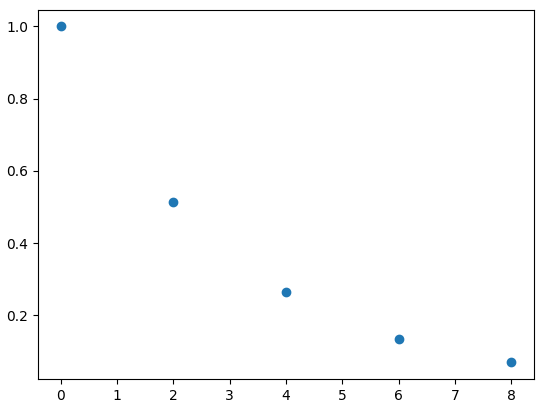
\includegraphics[width=0.4\textwidth]{../images/interp-data.png}
        \end{center}
        Y si quiero el valor en $x=3$? Eso se llama \emph{interpolación}\footnote{Extrapolación sería bajo 0 o sobre 8}
    }
    \begin{columns}
        \begin{column}{0.6\textwidth}
    \only<2->{
  {\tt\small
  > import numpy as np

  > import matplotlib.pyplot as plt

  > from scipy import interpolate

  > x = np.linspace(0,8,5)

  > y = np.exp(-x/3)

  > f = interpolate.interp1d(x, y, kind)

  > xnew = np.linspace(0,8,100)

  > ynew = f(xnew)
  }
    }
        \end{column}
        \begin{column}{0.39\textwidth}
            \only<2>{
            {\small
            \begin{center}
            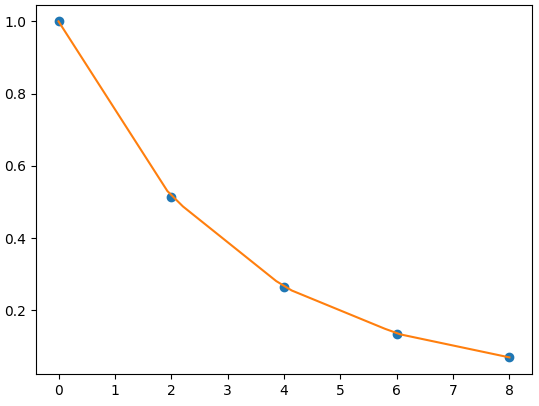
\includegraphics[width=\textwidth]{../images/interp-linear}
            \code{kind='linear'}
            \end{center}
            }
            }
            \only<3>{
            {\small
            \begin{center}
            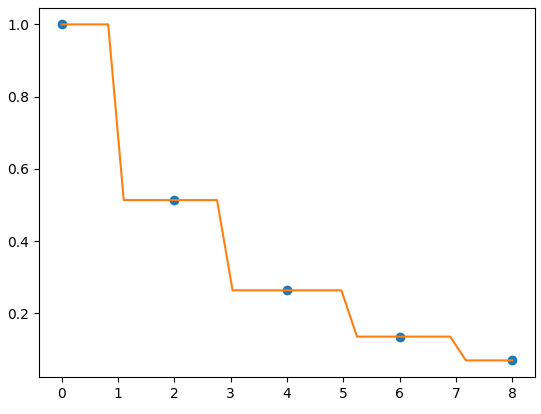
\includegraphics[width=\textwidth]{../images/interp-nearest}
            \code{kind='nearest'}
            \end{center}
            }
            }
            \only<4>{
            {\small
            \begin{center}
            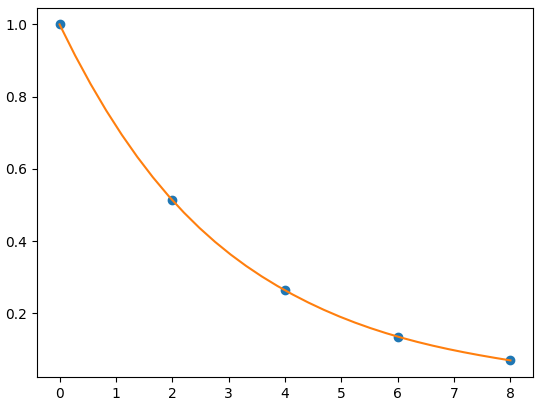
\includegraphics[width=\textwidth]{../images/interp-cubic}
            \code{kind='cubic'}
            \end{center}
            }
            }
        \end{column}
    \end{columns}
\end{frame}
%%%%%%%%%%%%%%%%%%%%%%%%%%%%%%%%%%%%%%%%%%%%%%%%%%%%%%%
\begin{frame}[t,fragile]\frametitle{Scipy: Solución de ecuaciones ($f(x)=0$)}
    \begin{small}
    $$ f(x) \coloneqq x + \sin x  = 0  $$
    \vspace{-0.5cm}
    \begin{columns}
        \begin{column}{0.49\textwidth}
    \begin{minted}{python}  
  from scipy.optimize import root_scalar 
  def f(x): return x+sin(2*pi*x)
  domx = np.linspace(-2,2,1000)
  domy = [f(x) for x in domx]
  x0,x1 = 3, -3
  sol = root_scalar(f, x0=x0, x1=x1)
  plt.scatter(sol.root, f(sol.root))
  plt.plot(domx, domy);plt.show()

    \end{minted}
        \end{column}
        \begin{column}{0.5\textwidth}
            \begin{flushright}
                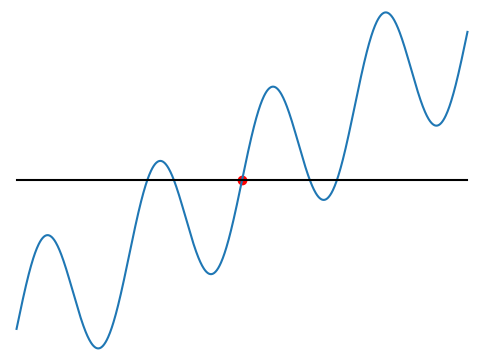
\includegraphics[width=0.7\textwidth]{../images/scipy-root.png}
            \end{flushright}
        \end{column}
    \end{columns}
    \pause\idea{Cómo obtener las otras soluciones?}
    \end{small}
\end{frame}
%%%%%%%%%%%%%%%%%%%%%%%%%%%%%%%%%%%%%%%%%%%%%%%%%%%%%%%
\begin{frame}[t,fragile]\frametitle{Scipy: Minimización}
    \begin{small}
    $$ \min_ x f(x) \coloneqq \sin^2 4x + x^2  = 0  $$
    \vspace{-0.5cm}
    \begin{columns}
        \begin{column}{0.49\textwidth}
    \begin{minted}{python}  
  from scipy.optimize import minimize_scalar 
  def f(x): return sin(4*x)**2 + x**2
  domx = np.linspace(-4,4,1000)
  domy = [f(x) for x in domx]
  sol = minimize_scalar(f)
  plt.scatter(sol.x, f(sol.x))
  plt.plot(domx, domy);plt.show()
    \end{minted}
        \end{column}
        \begin{column}{0.5\textwidth}
            \begin{flushright}
                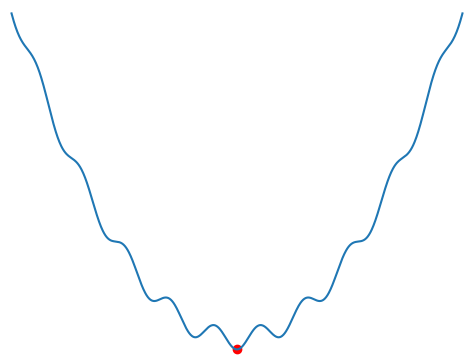
\includegraphics[width=0.7\textwidth]{../images/scipy-min.png}
            \end{flushright}
        \end{column}
    \end{columns}
    \end{small}
\end{frame}
%%%%%%%%%%%%%%%%%%%%%%%%%%%%%%%%%%%%%%%%%%%%%%%%%%%%%%%
\darkSlide{Soluciones numéricas NO SON exactas}
%%%%%%%%%%%%%%%%%%%%%%%%%%%%%%%%%%%%%%%%%%%%%%%%%%%%%%%
\begin{frame}\frametitle{Recap}
    \begin{itemize}
        \item Python tiene muchas librerías para hacer ciencia
        \item Algunas simples: \code{math}, \code{statistics}, \code{random}
        \item Otras complejas: \code{scipy}, \code{numpy}
        \item Scipy: interpolar, minimizar, resolver
    \end{itemize}
\end{frame}
%%%%%%%%%%%%%%%%%%%%%%%%%%%%%%%%%%%%%%%%%%%%%%%%%%%%%%%
\begin{frame}
    \maketitle
\end{frame}
%%%%%%%%%%%%%%%%%%%%%%%%%%%%%%%%%%%%%%%%%%%%%%%%%%%%%%%
\begin{frame}[fragile,noframenumbering]\frametitle{Mini ejercicios}
    \begin{itemize}
        \item Genere una sucesión de 0's y 1's que representan lanzamientos de monedas. Calcule indicadores estadísticos de sus datos usando \code{statistics}
        \item Considere la función $f(x)=\sin x$ y encuentre numéricamente un mínimo. Qué pasa con los otros mínimos? 
    \end{itemize}
\end{frame}
%%%%%%%%%%%%%%%%%%%%%%%%%%%%%%%%%%%%%%%%%%%%%%%%%%%%%%%
\end{document}
